%%% Local Variables:
%%% mode: latex
%%% TeX-master: "report_main"
%%% End:

\section{Part 1 - Mathematical modeling}
\subsection{Problem 1}

We use the helicopter model \cref{fig:helicopter_model} as our starting point for deriving the equations of motion.
\begin{figure}[hbp]
\caption{the helicopter model figure 7 from the assignment \cite[p.12]{assignment} with relevant distances drawn in.}
\label{fig:helicopter_model}
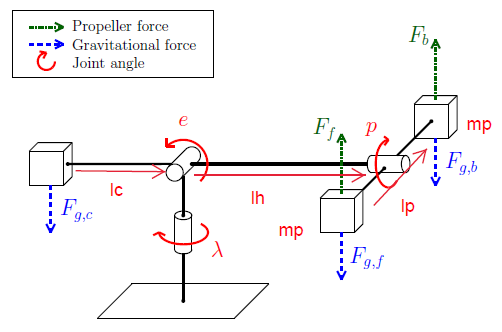
\includegraphics[width=\textwidth]{images/helicopter_model}
\end{figure}

The equation of motion for the pitch angle is found through the momentum around the pitch axis in the clockwise direction as shown in \cref{fig:helicopter_model}. It becomes:
\begin{align*}
J_p\ddot{p} &= l_p(F_{g,b} - F_b - F_{g,f} + F_f) \\
						&= l_p(m_pg - mp_g + K_fV_f - V_b) \\
						&= l_pK_f(V_f-V_b)
\end{align*}
Since $V_d = V_f-V_b$, we can write this as:
\begin{equation}
J_p\ddot{p} = l_pK_fVd
\end{equation}
Here, we can see that $L_1 = l_pK_f$.

The equation of motion for the elevation angle is found similarly through the momentum in the counter-clockwise direction around the elevation axis.
\begin{align*}
J_e\ddot{e} &= arm_cF_{g,c} - arm_h(F_{g,f}+F_{g_b} - K_fcos(p)(V_f + V_b))
\end{align*}
where $arm_c$ is the moment arm between the counterweight point mass and the elevation axis, and $arm_h$ is the moment arm between any of the two motor point masses and the elevation axis. As shown in \cref{fig:elevation_model}, $arm_c = l_ccos(e)$, and $arm_h = l_hcos(e)$. \todo{Husk at figuren må være som jeg (Daniel) har i notatene her, da er det 100 prosent tydelig hva $arm_c$ og $arm_h$ blir. Kan godt gjøre det enda litt mer detaljert.} We can immediately substitute $V_s = V_f + V_b$, and simplify:
\begin{align*}
J_e\ddot{e} &= l_ccos(e)m_cg - l_hcos(e)(2m_pg - K_fcos(p)V_s) \\
						&= cos(e)(l_cm_cg - 2l_hm_pg) + l_hK_fV_scos(e)cos(p)
\end{align*}
 Here, we have (as the author of the exercise) counted the cos(e) factor of the $V_s$ term as negligible, and set it to 1. \todo{Forklar hvor cos(p) kommer fra - og lag ny figur. Bruk denne til å forklare (2c)/(3) også.} The resulting equation has the form:
\begin{equation}
J_e\ddot{e} = g(l_cm_c - 2l_hm_p)cos(e) + l_hK_fV_scos(p)
\end{equation}
Note that $L_2 = g(l_cm_c-2l_hm_p)$, and $L_3 = l_hK_f$.

\begin{figure}[H]
\caption{the elevation model}
\label{fig:elevation_model}
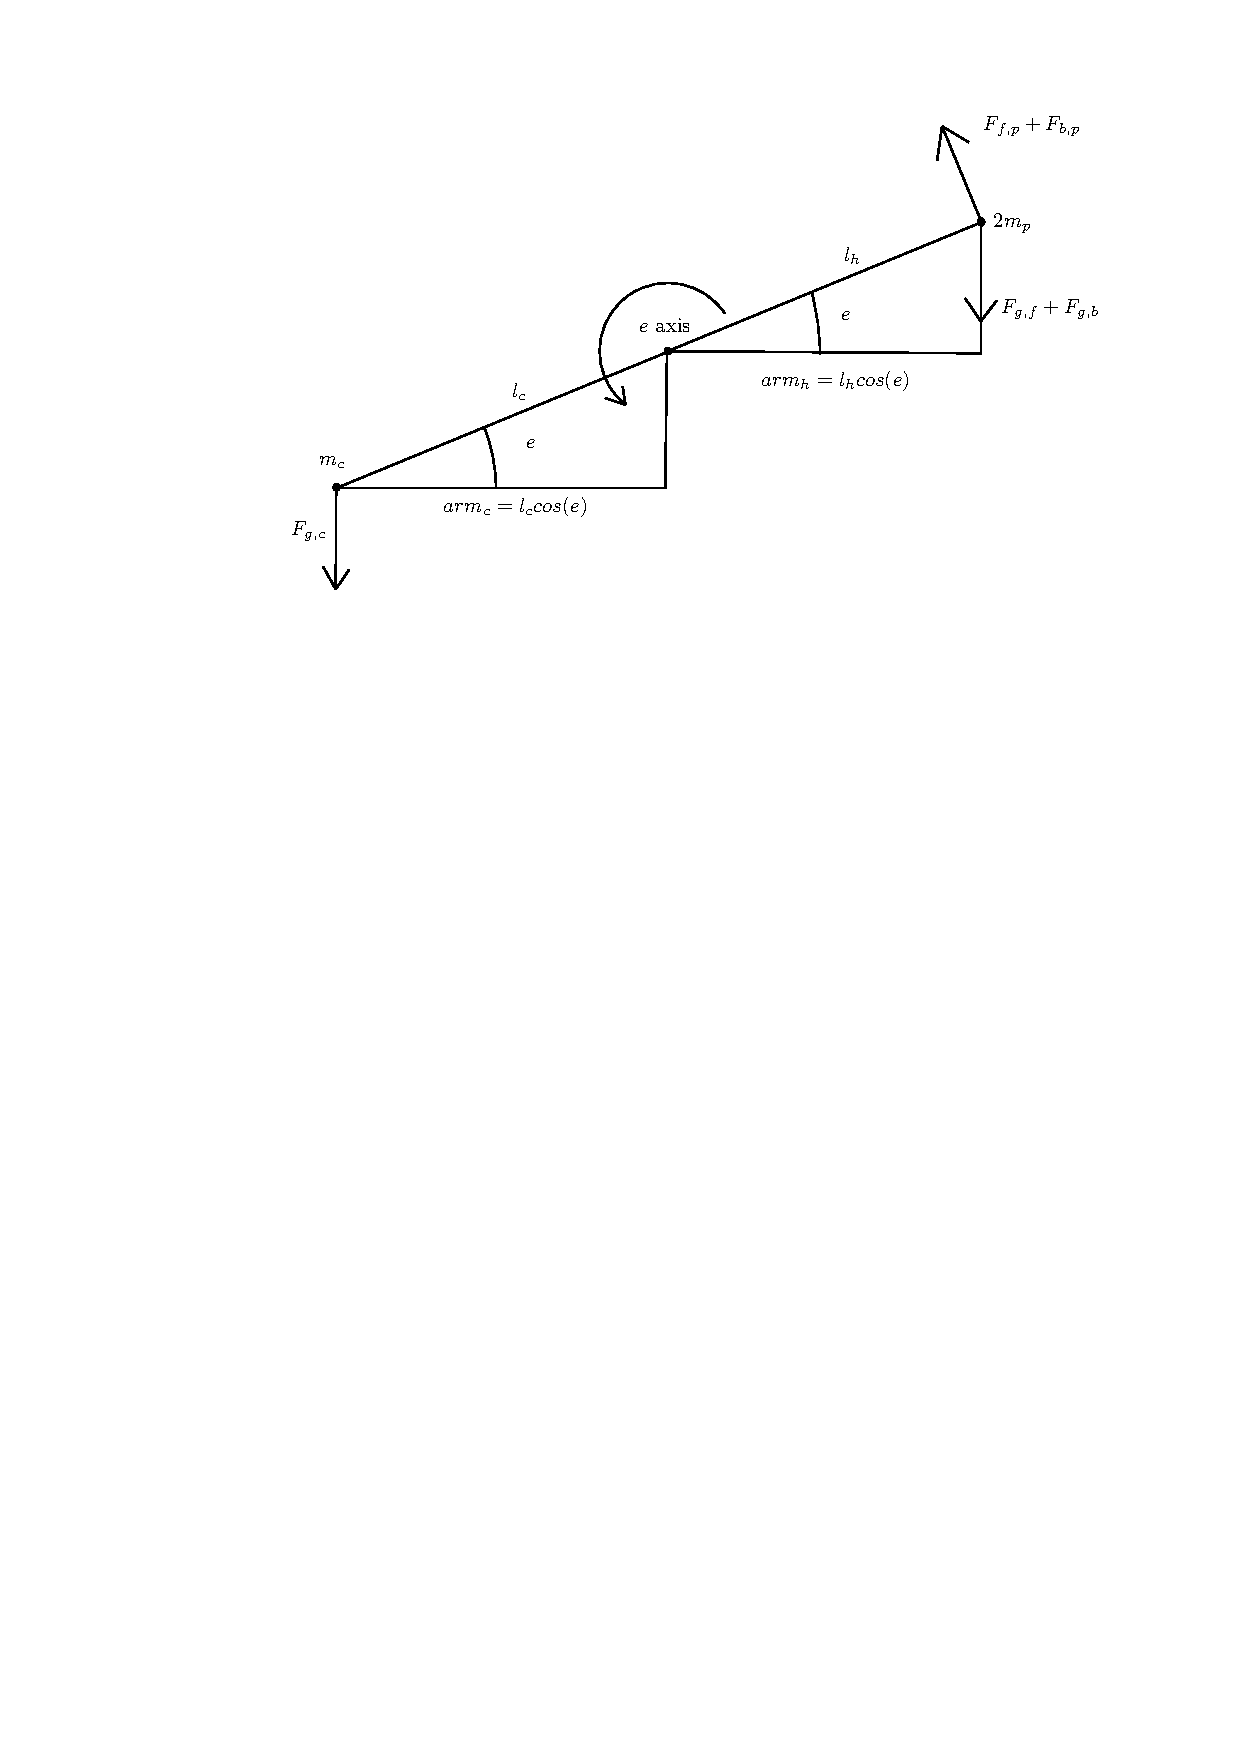
\includegraphics[width=0.5\textwidth]{images/elevation_model}
\end{figure}

Finally, the equation of motion for the travel angle is found through the momentum around the travel axis in the  clockwise direction. As seen in \cref{fig:elevation_model}, the only forces with a moment arm perpendicular to the travel axis are the components of the motor forces in the horizontal direction, which have length $arm_h = l_hcos(e)$. Furthermore, the horizontal components

\begin{figure}[H]
\caption{the pitch model}
\label{fig:pitch_model}
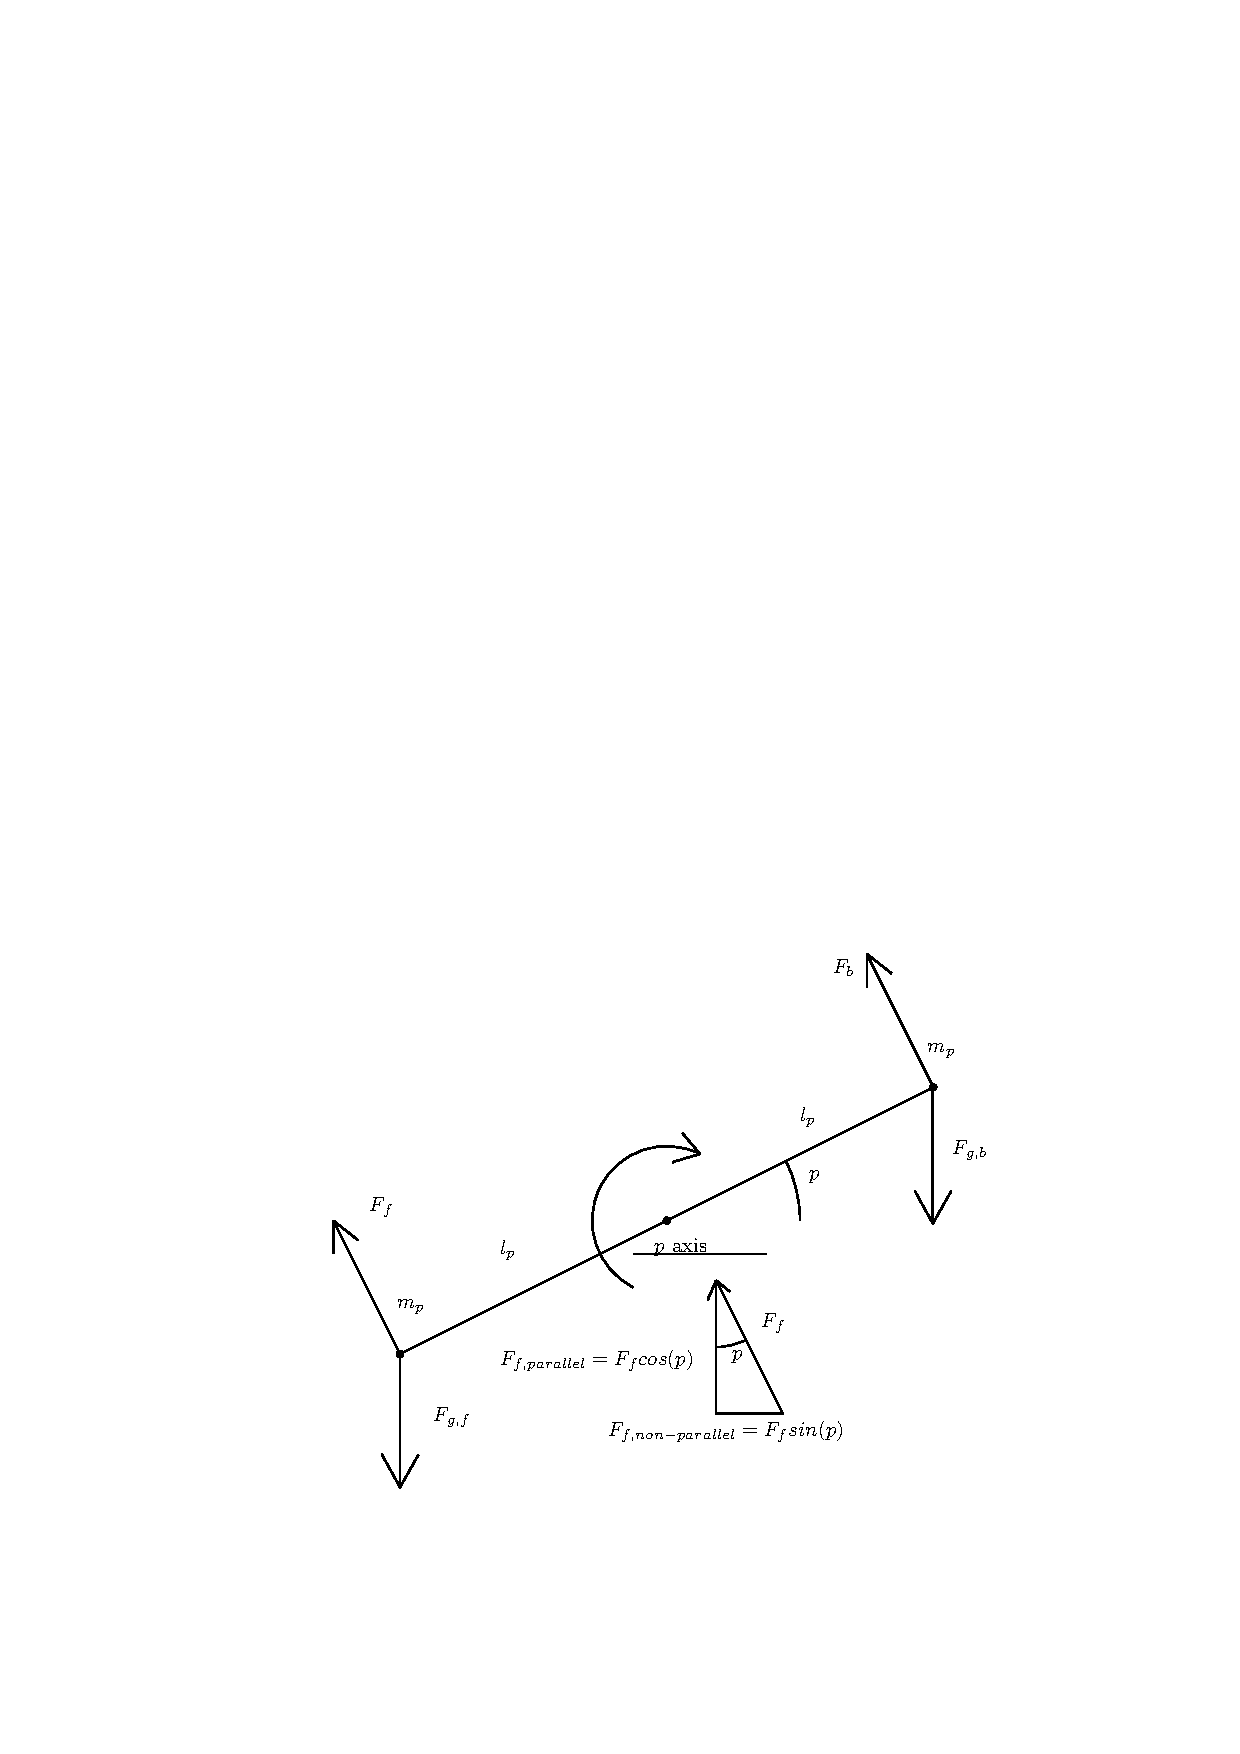
\includegraphics[width=0.5\textwidth]{images/pitch_model}
\end{figure}

\begin{align*}
J_\lambda\ddot{\lambda} &= arm_h
\end{align*}

The equations (1), (2), and (3) corresponds to (2a), (2b), and (2c) respectively of the assignment \cite[p.13]{assignment}

\subsection{Problem 2}
\subsection{Problem 3}
\subsection{Problem 4}
